\documentclass[11pt, uplatex, dvipdfmx]{jsarticle}
\usepackage{amsmath,amsfonts, bm, braket, setspace, emathEy, enumerate, graphicx}

\newcommand*{\ds}{\displaystyle}
\renewcommand*{\dlim}{\lim\limits} %emathEyを使わないなら\newcommand
\renewcommand*{\vec}[1]{\overrightarrow{\textrm{#1}}}

\resettagform


\pagestyle{plain}



\title{\Huge 線形代数 問題集}


\begin{document}

\maketitle
\thispagestyle{empty}

\newpage

\section{行列の演算}\label{sec:matrix}

\begin{enumerate}[\ref{sec:matrix}.1]
  \setlength{\itemsep}{1zh}
  
\item 次の行列 $A$ に対し,$A^n$ を求めよう.ただし,$n$ は自然数とする.

  \vspace{1ex}
  
  \begin{edaenumerate}<retusuu=3>[(1)]
  \item $A= \left[
      \begin{array}{rr}
        2 & 1\\
        0 & 2
      \end{array}
    \right]$

  \item $A=\left[
      \begin{array}{rrr}
        2 & 1 & 0\\
        0 & 2 & 0\\
        0 & 0 & 3
      \end{array}
    \right]$
    
  \item $A=\left[
      \begin{array}{rrr}
        2 & 1 & 0\\
        0 & 2 & 1\\
        0 & 0 & 2
      \end{array}
    \right]$
  \end{edaenumerate}\vspace{-2zh}

\item $B=\left[
    \begin{array}{rr}
      2 & 1\\
      0 & 2
    \end{array}
  \right], \; P=\left[
    \begin{array}{rr}
      3 & 4\\
      2 & 3
    \end{array}
  \right]$ とする.

  \vspace{1zh}
  
  \begin{enumerate}[(1)]
    \setlength{\itemsep}{1ex}
    
  \item $P^{-1}AP=B$ となる行列 $A$ を求めよう.

  \item 自然数 $n$ に対し,$A^n$ を求めよう.
  \end{enumerate}

\item $A=\left[
    \begin{array}{rr}
      -2 & 2\\
      5 & -3
    \end{array}
  \right]$ とする.

  \vspace{1zh}

  \begin{enumerate}[(1)]
    \setlength{\itemsep}{1ex}
    
  \item $A^2+5A-4E_2$ を計算しよう.

  \item (1) の結果を活用して $A^5$ を効率良く計算しよう.
  \end{enumerate}
  
\item 下図のような $5$ 個の空港 $1, 2, 3, 4 ,5$ を結ぶ航空路線がある.
  空港 $i$ から空港 $j$ への直通路線があるとき $a_{ij}=1$ とし,そうで
  ないとき $a_{ij}=0$ とする.ただし,$a_{ii}=0$ とする.
  \begin{figure}[h]
    \centering
    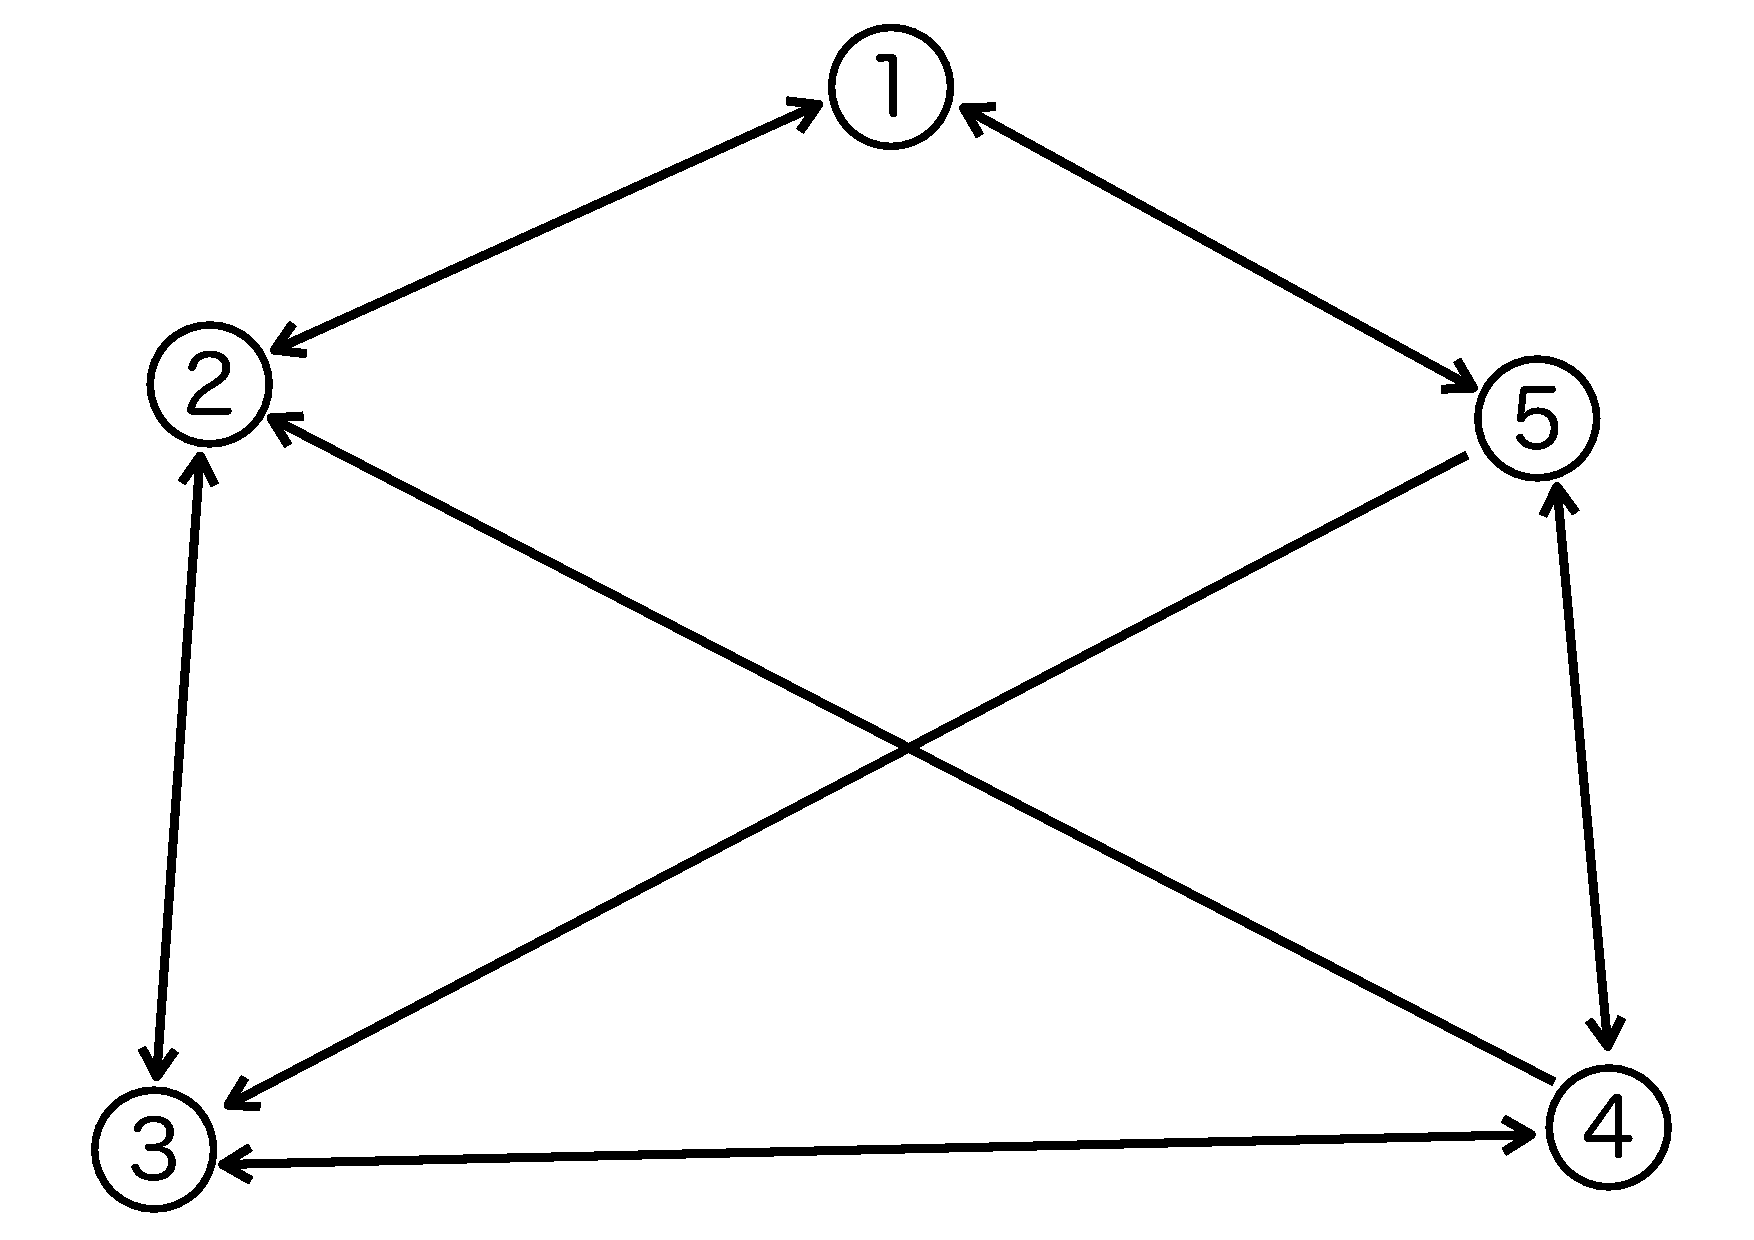
\includegraphics[width=6cm]{./pictures/routes.pdf}
  \end{figure}

  \begin{enumerate}[(1)]
    \setlength{\itemsep}{1ex}
    
  \item $a_{ij}$ を $(i,j)$ 成分とする $5$ 次正方行列 $A=\left[ a_{ij}\right]$ を具体的に書いてみよう.

  \item $A^2, A^3, A^4$ を計算しよう.

  \item $A^2$ の $(i,j)$ 成分は
    $a_{i1} a_{1j} + a_{i2}a_{2j} + a_{i3}a_{3j} + a_{i4}a_{4j} +
    a_{i5}a_{5j}$ であることから,この値が何を意味するか考えよう.

  \item 自然数 $n$ に対して $A^n$ の $(i,j)$ 成分が何を意味するか考えよう.

  \item 路線 $4 \to 2 \to 1 \to 5 \to 3$ のように,空港 $4$ から出発し
    て $4$ 回の移動($3$ 回の乗り継ぎ)で空港 $3$ に到着する路線の個数
    を求めよう.
  \end{enumerate}


\end{enumerate}

\section{行列の基本変形}\label{sec:transform}

以下の \ref{sec:transform}.\ref{trans:mul},
\ref{sec:transform}.\ref{trans:switch},
\ref{sec:transform}.\ref{trans:add}で定義する行列
$M_n(i;c), S_n(i,j), A_n(i,j;c)$ を(行の)基本行列という.


\begin{enumerate}[\ref{sec:transform}.1]
  \setlength{\itemsep}{1zh}
  
\item \label{trans:mul}$n$ 次単位行列 $E_n$ の $(i,i)$ 成分を $c$ で置き換えた行列を $M_n(i ; c)$ とする.

  \vspace{1ex}

  \begin{enumerate}[(1)]
    \setlength{\itemsep}{1ex}
    
  \item $M_3(1; 3), \; M_3(2; -2)$ を具体的に書いてみよう.

  \item $3$ 次正方行列 $A=\left[ a_{ij}\right]$ に対し,行列の
    積 $M_3(1;3)A$ と $M_3(2; -2) A$ を計算しよう.

  \item $M_n(i;c)$ を左から掛けることは何を意味するかを考えよ
    う.
  \end{enumerate}

\item \label{trans:switch}$n$ 次単位行列 $E_n$ の $(i,i)$ 成分と $(j,j)$ 成分を $0$ に,$(i,j)$ 成分
  と $(j,i)$ 成分を $1$ に置き換えた行列を $S_n(i,j) \; (i \neq j)$ とする.

  
  \vspace{1ex}

  \begin{enumerate}[(1)]
    \setlength{\itemsep}{1ex}
    
  \item $S_3(1,2), \; S_3(2, 3)$ を具体的に書いてみよう.

  \item $3$ 次正方行列 $A=\left[ a_{ij}\right]$ に対し,行列の
    積 $S_3(1,2)A$ と $S_3(2,3)A$ を計算しよう.

  \item $S_n(i,j)$ を左から掛けることは何を意味するかを考えよう.
  \end{enumerate}

\item \label{trans:add}$n$ 次単位行列 $E_n$ の $(i,j)$ 成分を $c$ で置き換えた行列
  を $A_n(i,j;c) \; (i \neq j)$ とする.

  \vspace{1ex}

  \begin{enumerate}[(1)]
    \setlength{\itemsep}{1ex}
    
  \item $A_3(1,2 ; 3), \; A_3(3, 2; -1)$ を具体的に書いてみよう.

  \item $3$ 次正方行列 $A=\left[ a_{ij}\right]$ に対し,行列の積 $A_3(1,2; 3)A$ と $A_3(3,2; -1)A$ を計算しよう.

  \item $A_n(i,j; c)$ を左から掛けることは何を意味するかを考えよう.
  \end{enumerate}

\item $A=\left[
    \begin{array}{rrr}
      0 & 3 & 6\\
      1 & 4 & 7\\
      2 & 5 & 8
    \end{array}
  \right]$ とし,$B=\left[ A \  \ E_3\right] = \left[
    \begin{array}{rrrrrr}
      0 & 3 & 6 & 1 & 0 & 0\\
      1 & 4 & 7 & 0 & 1 & 0\\
      2 & 5 & 8 & 0 & 0 & 1
    \end{array}
  \right]$ とする.

  \vspace{1zh}

  \begin{enumerate}[(1)]
    \setlength{\itemsep}{1ex}
    
  \item 行列の積 $S_3(1,2) B$ と $A_3(3,1; -2) S_3(1,2)B$ を計算しよう.

  \item $A$ の簡約化を $C$ とする.$PA=C$ となる $3$ 次正方行列 $P$ を求めよう.
    
  \end{enumerate}
  
\item $\bm{a}_1=\left[
    \begin{array}{r}
      1\\
      1\\
      2
    \end{array}
  \right], \; \bm{a}_2=\left[
    \begin{array}{r}
      1\\
      0\\
      1
    \end{array}
  \right], \; \bm{a}_3=\left[
    \begin{array}{r}
      2\\
      2\\
      1
    \end{array}
  \right], \quad A=\left[
    \begin{array}{ccc}
      \bm{a}_1 & \bm{a}_2 & \bm{a}_3
    \end{array}
  \right]$ とする.

  \vspace{1zh}

  \begin{enumerate}[(1)]
    \setlength{\itemsep}{1ex}

  \item 行列の積 ${}^{t}A A$ を計算しよう.
    
  \item 内積 $\bm{a}_i \cdot \bm{a}_j$ を $(i,j)$ 成分とする $3$ 次正方
    行列 $G=\left[ \bm{a}_i \cdot \bm{a}_j\right]$ を計算しよう.

  \item $L=A_3(3,1,-1) A_3\left(2,1,-\frac{1}{2}\right)$ とす
    る.行列の積 $LG$ と $L ({}^{t}A)$ を計算しよう.

  \item $B={}^{t}\left( L ({}^{t}A)\right)$ とする.行列の積 ${}^{t} B  B$ を計算しよう.
    
    
  \end{enumerate}
\end{enumerate}

\newpage

\section{連立1次方程式}\label{sec:system}

\begin{enumerate}[\ref{sec:system}.1]

  \setlength{\itemsep}{1zh}


\item 次の行列 $A, B$ に対して,$AX=B$ を満たす行列 $X$ を全て求めよう.

  \vspace{1ex}
  
  \begin{enumerate}[(1)]
    \setlength{\itemsep}{1zh}
    
  \item $A= \left[
      \begin{array}{rr}
        1 & 2\\
        3 & 4
      \end{array}
    \right] , \quad B=\left[
      \begin{array}{rr}
        9 & 5\\
        21 & 9
      \end{array}
    \right]$

  \item $A=\left[
      \begin{array}{ccc}
        1 & 2 & 3\\
        4 & 5 & 6\\
        7 & 8 & 9
      \end{array}
    \right], \quad B=\left[
      \begin{array}{rrr}
        -3 & 6 & 4\\
        3 & 9 & 16\\
        9 & 12 & 28
      \end{array}
    \right]$
  \end{enumerate}

\item 以下を満たす $3$ 次関
  数 $f(x)=a_0 + a_1 x + a_2 x^2 + a_3 x^3$ の係数を決定しよう.
  \[
    f(1)=1, \quad f(2)=2, \quad f'(1)=2, \quad f'(2)=3
  \]
  
\item $xy$ 平面において $a x^2 + bxy + cy^2 + dx + ey + f=0$ という形
  の $2$ 次方程式によって定まる曲線を $2$ 次曲線という.以下
  の $5$ 点 A, B, C, D, E を通る $2$ 次曲線の方程式を求めよう.
  \[
    \textrm{A}(3,-1), \quad \textrm{B}(2,2), \quad \textrm{C}(-4,-1),
    \quad \textrm{D}(-1,-2), \quad \textrm{E}(0,-4)
  \]

\item 4つの物質 A, B, Cを含む混合溶液 W, X, Y, Z がある.これら4つ
  の混合溶液を適切な割合で混ぜ合わせて新たな溶液 $\Omega$ を作りたい.
  以下の表は各溶液 W, X, Y, Z とこれから作りたい溶液 $\Omega$ の100gあ
  たりに含まれる物質 A, B, C の含有量(単位はg)を表したものである.
  各溶液を混ぜ合わせることで化学反応等による質量欠損は起きないものとし
  て,混ぜ合わせる溶液 W, X, Y, Z の適切な割合を求めよう.
  \begin{table}[h]
    \centering
    \begin{tabular}{ccccc|c}
      & W & X & Y & Z & $\Omega$\\ \hline
      A & 2.00 & 1.00 & 4.00 & 9.00 & 3.00\\ \hline
      B & 7.00 & 10.0 & 1.00 & 2.00 & 6.00\\ \hline  
      C & 4.00 & 8.00 & 10.0 & 7.00 & 7.00\\ 
    \end{tabular}
  \end{table}

  
\item $\bm{a}_1 = \left[
    \begin{array}{r}
      2\\
      2\\
      -1
    \end{array}
  \right], \; \bm{a}_2=\left[
    \begin{array}{r}
      1\\
      3\\
      -4
    \end{array}
  \right], \; \bm{b} = \left[
    \begin{array}{r}
      5\\
      2\\
      5
    \end{array}
  \right], \; A=\left[
    \begin{array}{cc}
      \bm{a}_1 & \bm{a}_2
    \end{array}
  \right]$ とする.
  
  \vspace{1zh}

  
  \begin{enumerate}[(1)]
    \setlength{\itemsep}{1ex}
    
  \item 連立1次方程式 $A\bm{x} = \bm{b}$ を解こう.

  \item 連立 $1$ 次方程式 ${}^{t}A A\bm{x} = {}^{t}A \bm{b}$ を解こう.

  \item (2) で求めた解 $\bm{x}$ に対して,空間ベクトルの内
    積 $(A\bm{x}) \cdot (A\bm{x} -\bm{b})$ を計算しよう.

  \item 空間ベクトル $A\bm{x}-\bm{b}$ の大きさの $2$ 乗 $|A\bm{x} - \bm{b}|^2$ が最小とな
    る $\bm{x}$ を求めよう.
  \end{enumerate}
  
\end{enumerate}

\newpage

\section{行列式}\label{sec:determinant}

\begin{enumerate}[\ref{sec:determinant}.1]
  \setlength{\itemsep}{1zh}
  
\item 

  \begin{enumerate}[(1)]
    \setlength{\itemsep}{1ex}
    
  \item O を原点とする $xy$ 平面上に $3$ 点 A$(a,c)$, B$(b,d)$,
    C$(a+b, c+d)$ があり,$\vec{OA}$ と $\vec{OB}$ は平行でないとする.
    平行四辺形 OACB と三角形 OAB の面積を求めよう.

  \item $2$ 次正方行列 $\left[
      \begin{array}{cc}
        a & b\\
        c & d
      \end{array}
    \right]$ の行列式を計算しよう.

  \item $5$ 点 P$(4,4)$, Q$(-2,6)$, R$(-5,1)$, S$(-3,-3)$, T$(5,-3)$ を
    頂点とする五角形 PQRST の面積を求めよう.
  \end{enumerate}

\item 空間ベクトル $\bm{a} = {}^{t}\left[
    \begin{array}{ccc}
      a_1 & a_2 & a_3
    \end{array}
  \right], \; \bm{b}=  {}^{t}\left[
    \begin{array}{ccc}
      b_1 & b_2 & b_3
    \end{array}
  \right]$ に対して
  \[
    \bm{a} \times \bm{b} = \left|
      \begin{array}{cc}
        a_2 & b_2\\
        a_3 & b_3
      \end{array}
    \right| \bm{e}_1 -\left|
      \begin{array}{cc}
        a_1 & b_1\\
        a_3 & b_3
      \end{array}
    \right|\bm{e}_2 + \left|
      \begin{array}{cc}
        a_1 & b_1\\
        a_2 & b_2
      \end{array}
    \right| \bm{e}_3 = \left|
      \begin{array}{ccc}
        a_1 & b_1 & \bm{e}_1\\
        a_2 & b_2 & \bm{e}_2\\
        a_3 & b_3 & \bm{e}_3
      \end{array}
    \right|
  \]
  を $\bm{a}$ と $\bm{b}$ の外積という.($\bm{e}_1, \bm{e}_2,
  \bm{e}_3$ を形式的に数のように扱って行列式を計算する)

  \vspace{1ex}

  \begin{enumerate}[(1)]
    \setlength{\itemsep}{1ex}
    
  \item 内積 $\bm{a} \cdot (\bm{a} \times \bm{b})$ と $\bm{b}\cdot ( \bm{a} \times \bm{b})$ を計算しよう.

  \item 空間ベクトル $\bm{a} \times \bm{b}$ の大きさ $|\bm{a} \times \bm{b}|$ を求めよう.

  \item 空間ベクトル $\bm{a}$ と $\bm{b}$ が張る平行四辺形の面積を求めよう.
    
  \end{enumerate}

\item ${}^{t}\bm{a}=\left[
    \begin{array}{ccc}
      a_1 & a_2 & a_3
    \end{array}
  \right], \; {}^{t}\bm{b}=\left[
    \begin{array}{ccc}
      b_1 & b_2 & b_3
    \end{array}
  \right], \; {}^{t}\bm{c} = \left[
    \begin{array}{ccc}
      c_1 & c_2 & c_3
    \end{array}
  \right]$ とする.

  \vspace{1zh}
  
  \begin{enumerate}[(1)]
    \setlength{\itemsep}{1ex}
    
  \item 空間ベクトル $\bm{a}$ と $\bm{b}$ と $\bm{a} \times \bm{b}$ が
    張る平行六面体の体積を求めよう.
    
  \item 空間ベクトル $\bm{a}$ と $\bm{b}$ と $\bm{c}$ が張る平行六面体の体積を求めよう.

  \item 空間ベクトルの内積 $(\bm{a} \times \bm{b}) \cdot \bm{c}$ を計算しよう.

  \item $3$ 次正方行列 $A=\left[
      \begin{array}{ccc}
        \bm{a} & \bm{b} & \bm{c}
      \end{array}
    \right]$ の行列式を計算しよう.
    
  \end{enumerate}
  
\item $xyz$ 空間の以下の $4$ 点 O, A, B, C を頂点とする四面
  体 OABC の体積と表面積を求めよう.
  \[
    \textrm{O}(0,0,0), \quad \textrm{A}(3,0,-3), \quad \textrm{B}(2,2,4), \quad \textrm{C}(-2,1,1)
  \]


\item $\bm{a}_1=\left[
    \begin{array}{r}
      1\\
      1\\
      2
    \end{array}
  \right], \; \bm{a}_2=\left[
    \begin{array}{r}
      1\\
      0\\
      1
    \end{array}
  \right], \; \bm{a}_3=\left[
    \begin{array}{r}
      2\\
      2\\
      1
    \end{array}
  \right], \; g_{ij} = \bm{a}_i \cdot \bm{a}_j \; (1 \leqq i,j \leqq 3)$ とする.

  \vspace{1zh}

  \begin{enumerate}[(1)]
    \setlength{\itemsep}{1ex}
    
  \item $\bm{b}_1 = \bm{a}_1, \quad \bm{b}_2= \left|
      \begin{array}{cc}
        g_{11} & g_{12}\\
        \bm{a}_1 & \bm{a}_2
      \end{array}
    \right|, \quad \bm{b}_3 = \left|
      \begin{array}{ccc}
        g_{11} & g_{12} & g_{13}\\
        g_{21} & g_{22} & g_{23}\\
        \bm{a}_1 & \bm{a}_2 & \bm{a}_3
      \end{array}
    \right|$ を計算しよう.

  \item $3$ 次正方行列 $B=\left[ \bm{b}_i \cdot \bm{b}_j\right]$ を計算しよう.
  \end{enumerate}
\end{enumerate}

\newpage

\section*{解答}

\begin{enumerate}[\ref{sec:matrix}.1]
  \setlength{\itemsep}{1zh}
  
\item \label{power}
  \begin{enumerate}[(1)]
    \setlength{\itemsep}{1ex}
    
  \item $A^2=\left[
      \begin{array}{rr}
        4 & 4\\
        0 & 4
      \end{array}
    \right], A^3=\left[
      \begin{array}{rr}
        8 & 12\\
        0 & 8
      \end{array}
    \right], A^4=\left[
      \begin{array}{rr}
        16 & 32\\
        0 & 16
      \end{array}
    \right]$ より $A^n=\left[
      \begin{array}{cc}
        2^n & n \cdot 2^{n-1}\\
        0 & 2^n
      \end{array}
    \right]$ と予想できる.実際,$n=1$ のときは明らかに正しくて,$n$ のとき正
    しいと仮定すると,$A^{n+1} =\left[
      \begin{array}{rr}
        2 & 1\\
        0 & 2
      \end{array}
    \right] \left[
      \begin{array}{cc}
        2^n & n \cdot 2^{n-1}\\
        0 & 2^n
      \end{array}
    \right] = \left[
      \begin{array}{cc}
        2^{n+1} & (n+1) \cdot 2^n\\
        0 & 2^{n+1}
      \end{array}
    \right]$ より $n+1$ のときも正しいので,数学的帰納法から予想は正しい.

  \item (1)の結果と行列の分割を用いて計算すると $A^n = \left[
      \begin{array}{ccr}
        2^n & n \cdot 2^{n-1} & 0\\
        0 & 2^n & 0\\
        0 & 0 & 3^n
      \end{array}
    \right]$.

  \item $N=\left[
      \begin{array}{ccc}
        0 & 1 & 0\\
        0 & 0 & 1\\
        0 & 0 & 0
      \end{array}
    \right]$ とすると $A=2E_3+N$ である.$2E_3N =
    N(2E_3)=2N$ より $2E_3$ と $N$ の積が可換だから二項展開が使える.
    さらに,$N^3=O$ なので $n \geqq 3$ のとき
    $A^n = (2E_3+N)^n = {\ds \sum_{i=0}^{n}}~ {}_n C_{i}
    (2E_3)^{n-i} N^i = 2^{n} E_3 + n \cdot 2^{n-1}N +
    \frac{n(n-1)}{2} \cdot 2^{n-2} N^2=\left[
      \begin{array}{ccc}
        2^n & n \cdot 2^{n-1} & n(n-1)\cdot 2^{n-3}\\
        0 & 2^n & n \cdot 2^{n-1}\\
        0 & 0 & 2^n
      \end{array}
    \right]$ である.これは $n=1,2$ でも明らかに正しい.
    
  \end{enumerate}

\item
  \begin{enumerate}[(1)]
    \setlength{\itemsep}{1ex}
    
  \item $A=PBP^{-1} = \left[
      \begin{array}{rr}
        3 & 4\\
        2 & 3
      \end{array}
    \right] \left[
      \begin{array}{rr}
        2 & 1\\
        0 & 2
      \end{array}
    \right] \left[
      \begin{array}{rr}
        3 & -4\\
        -2 & 3
      \end{array}
    \right] = \left[
      \begin{array}{rr}
        -4 & 9\\
        -4 & 8
      \end{array}
    \right]$
    
  \item
    $A^n = (PBP^{-1})^n = (PBP^{-1})(PBP^{-1}) \cdots (PBP^{-1}) =
    PB^n P^{-1}$ より,\ref{sec:matrix}.\ref{power}(1)から $A^n = P \left[
      \begin{array}{cc}
        2^n & n\cdot 2^{n-1}\\
        0 & 2^n
      \end{array}
    \right]P^{-1} = 2^{n-1} \left[
      \begin{array}{cc}
        2-6n & 9n\\
        -4n & 2+6n
      \end{array}
    \right]$.
  \end{enumerate}

\item
  \begin{enumerate}[(1)]
    \setlength{\itemsep}{1ex}
    
  \item $A^2+5A-4E_2=O$

  \item 前問より $A^2=4E_2-5A$
    なので,$A^5 =
    A(A^2)^2=A(16E_2-40A+25A^2)=A(116E_2-165A)=116A-165A^2=941A-660E_2 = \left[
      \begin{array}{rr}
        -2542 & 1882\\
        4705 & -3483
      \end{array}
    \right]$.
  \end{enumerate}

\item
  \begin{enumerate}[(1)]
    \setlength{\itemsep}{1ex}
    
  \item $A=\left[
      \begin{array}{rrrrr}
        0 & 1 & 0 & 0 & 1\\
        1 & 0 & 1 & 0 & 0\\
        0 & 1 & 0 & 1 & 0\\
        0 & 1 & 1 & 0 & 1\\
        1 & 0 & 1 & 1 & 0
      \end{array}
    \right]$

  \item $A^2=\left[
      \begin{array}{rrrrr}
        2 & 0 & 2 & 1 & 0\\
        0 & 2 & 0 & 1 & 1\\
        1 & 1 & 2 & 0 & 1\\
        2 & 1 & 2 & 2 & 0\\
        0 & 3 & 1 & 1 & 2
      \end{array}
    \right], \; A^3=\left[
      \begin{array}{rrrrr}
        0 & 5 & 1 & 2 & 3\\
        3 & 1 & 4 & 1 & 1\\
        2 & 3 & 2 & 3 & 1\\
        1 & 6 & 3 & 2 & 4\\
        5 & 2 & 6 & 3 & 1
      \end{array}
    \right], \; A^4=\left[
      \begin{array}{rrrrr}
        8 & 3 & 10 & 4 & 2 \\
        2 & 8 & 3 & 5 & 4 \\
        4 & 7 & 7 & 3 & 5 \\
        10 & 6 & 12 & 7 & 3 \\
        3 & 14 & 6 & 7 & 8 
      \end{array}
    \right]$

  \item $i \to \ast \to j$ と,空港 $i$ から $2$ 回の移動($1$ 回の乗り継ぎ)
    で空港 $j$ に到着する路線の個数

  \item 空港 $i$ から $n$ 回の移動($n-1$ 回の乗り継ぎ)で空港 $j$ に到
    着する路線の個数

  \item $A^4$ の $(4,3)$ 成分なので,(2) より $12$ 個.
  \end{enumerate}
\end{enumerate}

\vspace{1zh}

\begin{enumerate}[\ref{sec:transform}.1]
  \setlength{\itemsep}{1zh}
  
\item
  \begin{enumerate}[(1)]
    \setlength{\itemsep}{1ex}
    
  \item $M_3(1;3)=\left[
      \begin{array}{ccc}
        3 & 0 & 0\\
        0 & 1 & 0\\
        0 & 0 & 0
      \end{array}
    \right], \quad M_3(2;-2)=\left[
      \begin{array}{rrr}
        1 & 0 & 0\\
        0 & -2 & 0\\
        0 & 0 & 1
      \end{array}
    \right]$

  \item $M_3(1;3)A=\left[
      \begin{array}{rrr}
        3a_{11} & 3 a_{12} & 3 a_{13}\\
        a_{21} & a_{22} & a_{23}\\
        a_{31} & a_{32} & a_{33}
      \end{array}
    \right], \quad M_3(2;-2)A=\left[
      \begin{array}{rrr}
        a_{11} & a_{12} & a_{13}\\
        -2a_{21} & -2a_{22} & -2a_{23}\\
        a_{31} & a_{31} & a_{33}
      \end{array}
    \right]$

  \item 右の行列に行基本変形「$i$ 行目を $c$ 倍する」を適用することを意味する.
  \end{enumerate}

\item
  \begin{enumerate}[(1)]
    \setlength{\itemsep}{1ex}
    
  \item $S_3(1,2)=\left[
      \begin{array}{rrr}
        0 & 1 & 0\\
        1 & 0 & 0\\
        0 & 0 & 1
      \end{array}
    \right], \quad S_3(2,3) = \left[
      \begin{array}{rrr}
        1 & 0 & 0\\
        0 & 0 & 1\\
        0 & 1 & 0
      \end{array}
    \right]$

  \item $S_3(1,2)A=\left[
      \begin{array}{rrr}
        a_{21} & a_{22} & a_{23}\\
        a_{11} & a_{12} & a_{13}\\
        a_{31} & a_{3,2} & a_{33}
      \end{array}
    \right], \quad S_3(2,3) A = \left[
      \begin{array}{rrr}
        a_{11} & a_{12} & a_{13}\\
        a_{31} & a_{32} & a_{33}\\
        a_{21} & a_{22} & a_{23}
      \end{array}
    \right]$

  \item 右の行列に行基本変形「第 $i$ 行と第 $j$ 行を入れ替える」を適用することを意味する.
  \end{enumerate}

\item
  \begin{enumerate}[(1)]
    \setlength{\itemsep}{1ex}
    
  \item $A_3(1,2;3)=\left[
      \begin{array}{rrr}
        1 & 3 & 0\\
        0 & 1 & 0\\
        0 & 0 & 1
      \end{array}
    \right], \quad A_3(3,2,-1)=\left[
      \begin{array}{rrr}
        1 & 0 & 0\\
        0 & 1 & 0\\
        0 & -1 & 1
      \end{array}
    \right]$
    
  \item $S_3(1,2;3)A=\left[
      \begin{array}{ccc}
        a_{11}+3a_{21} & a_{12}+3a_{22} & a_{13}+3a_{23}\\
        a_{21} & a_{22} & a_{23}\\
        a_{31} & a_{32} & a_{33}
      \end{array}
    \right]$ \vspace{1ex}

    $S_3(3,2;-1)A=\left[
      \begin{array}{ccc}
        a_{11} & a_{12} & a_{13}\\
        a_{21} & a_{22} & a_{23}\\
        a_{31}-a_{21} & a_{32} -a_{22} & a_{33}-a_{23}
      \end{array}
    \right]$
    
  \item 右の行列に行基本変形「第 $i$ 行に第 $j$ 行の $c$ 倍を加える」を適用することを意味する.
  \end{enumerate}

\item
  \begin{enumerate}[(1)]
    \setlength{\itemsep}{1ex}
    
  \item   $S_3(1,2)B=\left[
      \begin{array}{rrrrrr}
        1 & 4 & 7 & 0 & 1 & 0\\
        0 & 6 & 1 & 0 & 1 & 0\\
        2 & 5 & 8 & 0 & 0 & 1
      \end{array}
    \right]$ \vspace{1ex}

    $A_3(3,1;-2) S_3(1,2)B = \left[
      \begin{array}{rrrrrr}
        1 & 4 & 7 & 0 & 1 & 0\\
        0 & 3 & 6 & 1 & 0 & 0\\
        0 & -3 & -6 & 0 & -2 & 1
      \end{array}
    \right]$


  \item $PB = \left[PA \; PE_3\right] = \left[ C \ P\right]$ は簡約行列な
    ので,$B$ を簡約化すればよい.(1)を続けて
    \[
      \renewcommand{\arraystretch}{1.1}
      B \to \left[
        \begin{array}{rrrrrr}
          1 & 4 & 7 & 0 & 1 & 0\\
          0 & 3 & 6 & 1 & 0 & 0\\
          0 & -3 & -6 & 0 & -2 & 1
        \end{array}
      \right] \to \cdots \to \left[
        \begin{array}{rrrrrr}
          1 & 0 & -1 & 0 & -\frac{5}{3} & \frac{4}{3}\\
          0 & 1 & 2 & 0 & \frac{2}{3} & -\frac{1}{3}\\
          0 & 0 & 0 & 1 & -2 & 1
        \end{array}
      \right]
      \renewcommand{\arraystretch}{1}
    \]
    より $P=\left[
      \begin{array}{rrr}
        0 & -\frac{5}{3} & \frac{4}{3}\\
        0 & \frac{2}{3} & -\frac{1}{3}\\
        1 & -2 & 1
      \end{array}
    \right]$.
  \end{enumerate}


\item
  \begin{enumerate}[(1)]
    \setlength{\itemsep}{1ex}
    
  \item ${}^{t}AA = \left[
      \begin{array}{rrr}
        6 & 3 & 6\\
        3 & 2 & 3\\
        6 & 3 & 9
      \end{array}
    \right]$

  \item $\bm{a}_i \cdot \bm{a}_j = {}^{t}\bm{a}_i \bm{a}_j$ なの
    で,$G= \left[
      \begin{array}{ccc}
        {}^{t}\bm{a}_1 \bm{a}_1 & {}^{t} \bm{a}_1 \bm{a}_2 & {}^{t}\bm{a}_1 \bm{a}_3\\
        {}^{t}\bm{a}_2 \bm{a}_1 & {}^{t}\bm{a}_2 \bm{a}_2 & {}^{t}\bm{a}_2 \bm{a}_3\\
        {}^{t}\bm{a}_3\bm{a}_1 & {}^{t}\bm{a}_3\bm{a}_2 & {}^{t}\bm{a}_3 \bm{a}_3
      \end{array}
    \right]=\left[
      \begin{array}{c}
        {}^{t}\bm{a}_1\\
        {}^{t}\bm{a}_2\\
        {}^{t}\bm{a}_3
      \end{array}
    \right] \left[
      \begin{array}{ccc}
        \bm{a}_1 & \bm{a}_2 & \bm{a}_3
      \end{array}
    \right]= {}^{t}AA = \left[
      \begin{array}{ccc}
        6 & 3 & 6\\
        3 & 2 & 3\\
        6 & 3 & 9
      \end{array}
    \right]$.

  \item $L=\left[
      \begin{array}{rrr}
        1 & 0 & 0\\
        -\frac{1}{2} & 1 & 0\\
        -1 & 0 & 1
      \end{array}
    \right]$ より,$LG=\left[
      \begin{array}{rrr}
        6 & 3 & 6\\
        0 & \frac{1}{2} & 0\\
        0 & 0 & 3
      \end{array}
    \right], \quad L({}^{t}A) = \left[
      \begin{array}{rrr}
        1 & 1 & 2\\
        \frac{1}{2} & -\frac{1}{2} & 0\\
        1 & 1 & -1
      \end{array}
    \right]$.

  \item ${}^{t} B B = \left[
      \begin{array}{rrr}
        1 & 1 & 2\\
        \frac{1}{2} & -\frac{1}{2} & 0\\
        1 & 1 & -1
      \end{array}
    \right] \left[
      \begin{array}{rrr}
        1 & \frac{1}{2} & 1\\
        1 & -\frac{1}{2} & 1\\
        2 & 0 & -1
      \end{array}
    \right] = \left[
      \begin{array}{rrr}
        6 & 0 & 0\\
        0 & \frac{1}{2} & 0\\
        0 & 0 & 3
      \end{array}
    \right]$.

    \vspace{1zh}
    
    補足:$B=\left[ \bm{b}_1 \ \bm{b}_2 \ \bm{b}_3 \right]$ とおけ
    ば,$\left[ \bm{b}_i \cdot \bm{b}_j\right] = {}^{t}BB$ なの
    で,(4) の結果は
    $\bm{b}_1 \cdot \bm{b}_2 = \bm{b}_1 \cdot \bm{b}_3 = \bm{b}_2
    \cdot \bm{b}_3=0$ を意味する.つまり,$\bm{b}_1, \bm{b}_2,
    \bm{b}_3$
    は互いに直交する.$3 \times 6$ 行列 $\left[
      \begin{array}{cc}
        G & {}^{t}A
      \end{array}
    \right]$ に左 $3$ 列が上三角行列になるまで「ある行に別の行の定数
    倍を加える」という行基本変形を適宜繰り返したのが $L\left[
      \begin{array}{cc}
        G & {}^{t}A
      \end{array}
    \right] =\left[
      \begin{array}{cc}
        LG & L({}^{t}A)
      \end{array}
    \right] = \left[
      \begin{array}{cc}
        LG & {}^{t}B
      \end{array}
    \right]$ である.これは与えれたベクトルたちから互いに直交するベク
    トルたちを行列の行基本変形によって作り出している.
  \end{enumerate}
  
\end{enumerate}


\begin{enumerate}[\ref{sec:system}.1]
  \setlength{\itemsep}{1zh}
  
\item
  \begin{enumerate}[(1)]
    \setlength{\itemsep}{1ex}

  \item $X=\left[
      \begin{array}{cc}
        \bm{x}_1 & \bm{x}_2
      \end{array}
    \right]$ とおくと,
    \[
      AX = B \quad \Longleftrightarrow \quad \left[
        \begin{array}{cc}
          1 & 2\\
          3 & 5
        \end{array}
      \right] \bm{x}_1 = \left[
        \begin{array}{r}
          9\\
          21
        \end{array}
      \right] \text{ かつ } \left[
        \begin{array}{cc}
          1 & 2\\
          3 & 4
        \end{array}
      \right] \bm{x}_2 = \left[
        \begin{array}{r}
          5\\
          9
        \end{array}
      \right]
    \]
    なので,$2$ 個の連立1次方程式を同時に解くために,$\left[
      \begin{array}{cc}
        A & B
      \end{array}
    \right]$ を簡約化すればよい.$\left[
      \begin{array}{cc}
        A & B
      \end{array}
    \right] = \left[
      \begin{array}{rrrr}
        1 & 2 & 9 & 5\\
        3 & 4 & 21 & 9
      \end{array}
    \right] \to \left[
      \begin{array}{rrrr}
        1 & 0 & 3 & -1\\
        0 & 1 & 3 & 3
      \end{array}
    \right]$ より $X=\left[
      \begin{array}{rr}
        3 & -1\\
        3 & 3
      \end{array}
    \right]$.

  \item $X=\left[
      \begin{array}{ccc}
        \bm{x}_1 & \bm{x}_2 & \bm{x}_3
      \end{array}
    \right], B=\left[
      \begin{array}{ccc}
        \bm{b}_1 & \bm{b}_2 & \bm{b}_3
      \end{array}
    \right]$ とおくと,
    \[
      AX=B \quad \Longleftrightarrow \quad A\bm{x}_1 = \bm{b}_1
      \text{ かつ } A\bm{x}_2 = \bm{b}_2 \text{ かつ }
      A\bm{x}_3=\bm{b}_3
    \]
    なので,$3$ 個の連立1次方程式を同時解くために $\left[
      \begin{array}{cc}
        A & B
      \end{array}
    \right]$ を簡約化すればよい.
    $\left[
      \begin{array}{cc}
        A & B
      \end{array}
    \right] = \left[
      \begin{array}{rrrrrr}
        1 & 2 & 3 & -3 & 6 & 4\\
        4 & 5 & 6 & 3 & 9 & 16\\
        7 & 8 & 9 & 9 & 12 & 28
      \end{array}
    \right] \to  \left[
      \begin{array}{rrrrrr}
        1 & 0 & -1 & 7 & -4 & 4\\
        0 & 1 & 2 & -5 & 5 & 0\\
        0 & 0 & 0 & 0 & 0 & 0
      \end{array}
    \right]$ なので
    \[
      \begin{aligned}
        A\bm{x}_1 = \bm{b}_1 & \Leftrightarrow \left[
                               \begin{array}{rrr}
                                 1 & 0 & -1\\
                                 0 & 1 & 2
                               \end{array}
                               \right] \bm{x}_1 = \left[
                               \begin{array}{r}
                                 7\\
                                 -5
                               \end{array}
                               \right] \Leftrightarrow \bm{x}_1 = \left[
                               \begin{array}{r}
                                 7\\
                                 -5\\
                                 0
                               \end{array}
                               \right] + c_1 \left[
                               \begin{array}{r}
                                 1\\
                                 -2\\
                                 1
                               \end{array}
                               \right]\\
        A\bm{x}_2 = \bm{b}_2 & \Leftrightarrow \left[
                               \begin{array}{rrr}
                                 1 & 0 & -1\\
                                 0 & 1 & 2
                               \end{array}
                               \right] \bm{x}_2 = \left[
                               \begin{array}{r}
                                 -4\\
                                 5
                               \end{array}
                               \right] \Leftrightarrow \bm{x}_2 = \left[
                               \begin{array}{r}
                                 -4\\
                                 5\\
                                 0
                               \end{array}
                               \right] + c_2 \left[
                               \begin{array}{r}
                                 1\\
                                 -2\\
                                 1
                               \end{array}
                               \right]\\
        A\bm{x}_3=\bm{b}_3 & \Leftrightarrow \left[
                             \begin{array}{rrr}
                               1 & 0 & -1\\
                               0 & 1 & 2
                             \end{array}
                             \right] \bm{x}_3 = \left[
                             \begin{array}{r}
                               4\\
                               0
                             \end{array}
                             \right] \Leftrightarrow \bm{x}_3=\left[
                             \begin{array}{r}
                               4\\
                               0\\
                               0
                             \end{array}
                             \right] + c_3\left[
                             \begin{array}{r}
                               1\\
                               -2\\
                               1
                             \end{array}
                             \right]
      \end{aligned}
    \]
    より $X=\left[
      \begin{array}{rrr}
        7 & -4 & 4\\
        -5 & 5 & 0\\
        0 & 0 & 0
      \end{array}
    \right] + c_1 \left[
      \begin{array}{rrr}
        1 & 0 & 0\\
        -2 & 0 & 0\\
        1 & 0 & 0
      \end{array}
    \right] + c_2 \left[
      \begin{array}{rrr}
        0 & 1 & 0\\
        0 & -2 & 0\\
        0 & 1 & 0
      \end{array}
    \right] + c_3\left[
      \begin{array}{rrr}
        0 & 0 & 1\\
        0 & 0 & -2\\
        0 & 0 & 1
      \end{array}
    \right]$.
  \end{enumerate}

  
  
\item $\begin{cases}
  f(1) = a_0 + a_1 + a_2 + 3a_3=1\\
  f(2) = a_0 + 2a_1 + 4a_2 + 9a_3=2\\
  f'(1) = a_1+2a_2+3a_3=2\\
  f'(2) = a_1+4a_2+12a_3=3
\end{cases}$ を解いて $f(x) = -8 + 19x -13x^2+3x^3$.

\item $f(x,y) = ax^2+bxy+cy^2+dx+ey+f$ とおく.同次形連立1次方程式
  \[
    \begin{cases}
      f(3,-1) = 9a-3b+c+3d-e+f=0\\
      f(2,2)=4a+4b+4c+ed+ee+f=0\\
      f(-4,-1)=16a+4b+c-4d-e+f=0\\
      f(-1,-2)=a+2b+4c-d-2e+f=0\\
      f(0,-4)=16c-4e+f=0
    \end{cases}
  \]
  を解いて $(a,b,c,d,e,f) = ( k, 6k, -k, 7k, -9k, -20k)$ を得る.明らか
  に $k\neq 0$ なので,求める $2$ 次曲線の方程式は $x^2+6xy-y^2+7x-9y-20=0$.
  
\item W, X, Y, Z をそれぞれ $w, x, y, z$ ずつ混ぜる.$\Omega$ に含まれ
  る A, B, C の割合からそれぞれ
  \[
    \begin{aligned}
      &\frac{ \frac{2}{100}w + \frac{1}{100}x + \frac{4}{100}y +
      \frac{9}{100}z}{w+x+y+z} = \frac{3}{100}, \quad 
      \frac{\frac{7}{100}w+\frac{10}{100}x+\frac{1}{100}y
      + \frac{2}{100}z}{w+x+y+z}=\frac{6}{100},\\
      &\frac{\frac{4}{100}w+\frac{8}{100}x+\frac{10}{100}y+\frac{7}{100}z}{w+x+y+z}
      =\frac{7}{100}
    \end{aligned}
  \]
  が成り立つ.これらを整理して得られる同次形連立1次方程式 $\begin{cases}
      w+2x-y-6z=0\\
      w+4x-5y-4z=0\\
      3w-x-3y=0
  \end{cases}$ を解いて $(w,x,y,z) = (37c, 36c, 25c,  14c)$ を得る.
  明らかに $c \neq 0$ なので,W, X, Y,
  Z を $37c:36c:25c:14c = 37:36:25:14$ の割合で混ぜればよい.


\item
  \begin{enumerate}[(1)]
    \setlength{\itemsep}{1ex}
    
  \item 解はない.

  \item ${}^{t} A A \bm{x} = {}^{t}A\bm{b} \Leftrightarrow \left[
      \begin{array}{rr}
        9 & 12\\
        12 & 26
      \end{array}
    \right] \bm{x} = \left[
      \begin{array}{r}
        9\\
        -9
      \end{array}
    \right]$ より解は $\bm{x} = \left[
      \begin{array}{r}
        \frac{19}{5}\\
        -\frac{21}{10}
      \end{array}
    \right]$.
      
    
  \item $(A\bm{x}) \cdot (A\bm{x}-\bm{b}) = \left[
      \begin{array}{r}
        \frac{11}{2}\\
        \frac{13}{10}\\
        \frac{23}{5}
      \end{array}
    \right] \cdot \left[
      \begin{array}{r}
        \frac{1}{2}\\
        -\frac{7}{10}\\
        -\frac{2}{5}
      \end{array}
    \right]=0$
    
  \item $\bm{x}=\left[
      \begin{array}{c}
        x_1\\
        x_2
      \end{array}
    \right]$ とおくと,$A\bm{x} = \left[
      \begin{array}{cc}
        \bm{a}_1 & \bm{a}_2
      \end{array}
    \right] \left[
      \begin{array}{c}
        x_1\\
        x_2
      \end{array}
    \right] = x_1 \bm{a}_1 + x_2 \bm{a}_2$ なので,$A\bm{x}$ を位置ベク
    トルとする点を H とすれば,H は $\bm{a}_1$ と $\bm{a}_2$ が張る平面
    上にある.$\bm{b}$ を位置ベクトルとする点を B とすれば,$A\bm{x} -
    \bm{b} = \vec{BH}$ なので $\vec{OH}$ と $\vec{BH}$ が直交するとき,
    すなわち,$A\bm{x} \cdot (A\bm{x}-\bm{b})=0$ のと
    き $|\vec{OH}|=|A\bm{x}-\bm{b}|$ は最小となる.よって,(2), (3) よ
    り $\bm{x}=\left[
      \begin{array}{r}
        \frac{19}{5}\\
        -\frac{21}{10}
      \end{array}
    \right]$ のとき $|A\bm{x}-\bm{b}|^2$ は最小となる.

    \vspace{1zh}

    補足:(2) の $\bm{x}$ は (4) で見たように $|A\bm{x}-\bm{b}|^2$ を最
    小にするので,連立 $1$ 次方程式 $A\bm{x} = \bm{b}$ の最小 $2$ 乗解
    と呼ばれる.$A\bm{x} - \bm{b}$ が最も $\bm{0}$ に近づく $\bm{x}$ で
    という意味で,厳密が解は存在しない方程式 $A\bm{x}=\bm{b}$ の近似解
    として採用される.
  \end{enumerate}

\end{enumerate}

\begin{enumerate}[\ref{sec:determinant}.1]
  \setlength{\itemsep}{1zh}
  
\item \label{area}
  \begin{enumerate}[(1)]
    \setlength{\itemsep}{1ex}
    
  \item $\bm{a} = \vec{OA}, \, \bm{b} = \vec{OB}$ のなす角を $\theta$ とする.平行四辺
    形 OACB の面積を $S$ とすれば,
    \[
      \begin{aligned}
        S^2 &= \left( |\bm{a}| \bm{b}| \sin \theta\right)^2
              = |\bm{a}|^2 |\bm{b}|^2 ( 1-\cos^2\theta)
              =|\bm{a}|^2|\bm{b}|^2 - \left(|\bm{a}||\bm{b}|\cos\theta\right)^2
              =|\bm{a}|^2|\bm{b}|^2 - \left(\bm{a} \cdot \bm{b}\right)^2\\
        &= (a^2+c^2)(b^2+d^2) - (ab+cd)^2 = (ad-bc)^2
      \end{aligned}
    \]
    より,平行四辺形 OACB の面積は $|ad-bc|$ で,三角形 OAB の面積
    は $\frac{S}{2}= \frac{|ad-bc|}{2}$.
    
  \item $\det \left[
      \begin{array}{cc}
        a & b\\
        c & d
      \end{array}
      \right] = ad-bc$

    \item $3$ つの三角形 PQR, PRS, PST の面積を合わせればよ
      い.(1), (2) から,三角形 PQR の面積は,$\frac{1}{2}\left| \det\left[
          \begin{array}{cc}
            \vec{PQ} & \vec{PR}
          \end{array}
        \right]\right| = \frac{1}{2} \left|\det\left[
          \begin{array}{rr}
            -6 & -9\\
             2 &  -3  
          \end{array}
        \right]\right|=18$ である.同様に,三角形 PRS の面積
      は $\frac{1}{2}\left| \det\left[
          \begin{array}{cc}
            \vec{PR} & \vec{PS}
          \end{array}
          \right] \right| = \frac{1}{2}\left| \det\left[
            \begin{array}{rr}
              -9 & -7\\
              -3 & -7
            \end{array}
          \right] \right| = 21$ で,三角形 PST の面積
        は $\frac{1}{2}\left| \det\left[
              \begin{array}{cc}
                \vec{PS} & \vec{PT}
              \end{array}
            \right]\right| = \frac{1}{2}\left| \det\left[
              \begin{array}{rr}
                -7 & 1\\
                -7 & -7
              \end{array}
            \right]\right| = 28$ である.よって,五角形 PQRST の面積
          は $18+21+28=67$.
      
  \end{enumerate}

\item \label{crossproduct}
  \begin{enumerate}[(1)]
    \setlength{\itemsep}{1ex}
    
  \item $\bm{a} \cdot (\bm{a} \times \bm{b}) = a_1 \left|
      \begin{array}{rr}
        a_2 & b_2\\
        a_3 & b_3
      \end{array}
    \right| - a_2\left|
      \begin{array}{rr}
        a_1 & b_1\\
        a_3 & b_3
      \end{array}
    \right| + a_3\left|
      \begin{array}{rr}
        a_1 & b_1\\
        a_2 & b_2
      \end{array}
    \right| = \left|
      \begin{array}{rrr}
        a_1 & b_1 & a_1\\
        a_2 & b_2 & a_2\\
        a_3 & b_3 & a_3
      \end{array}
    \right| =0$

    $\bm{b} \cdot (\bm{a} \times \bm{b}) = b_1 \left|
      \begin{array}{rr}
        a_2 & b_2\\
        a_3 & b_3
      \end{array}
    \right| - b_2\left|
      \begin{array}{rr}
        a_1 & b_1\\
        a_3 & b_3
      \end{array}
    \right| + b_3\left|
      \begin{array}{rr}
        a_1 & b_1\\
        a_2 & b_2
      \end{array}
    \right| = \left|
      \begin{array}{rrr}
        a_1 & b_1 & b_1\\
        a_2 & b_2 & b_2\\
        a_3 & b_3 & b_3
      \end{array}
    \right| =0$

    
  \item  $\bm{a} \times \bm{b} = {}^{t} \left[
      \begin{array}{ccc}
        a_2 b_3 - a_3 b_2 & -(a_1b_3-a_3b_a) & a_1b_2-a_2b_1
      \end{array}
      \right]$ なので
    \[
      \begin{aligned}
        |\bm{a} \times \bm{b}| &= \sqrt{(a_2b_3-a_3b_2)^2 + (a_1b_3-a_3b_1)^2 + (a_1b_2-a_2b_1)^2}\\
        &= \sqrt{(a_1^2+a_2^2+a_3^2)(b_1^2+b_2^2+b_3^2) - (a_1b_1+a_2b_2+a_3b_3)^2}.
      \end{aligned}
    \]

  \item \ref{sec:determinant}.\ref{area}(1) と同様
    に,$\bm{a}$ と $\bm{b}$ が張る平行四辺形の面積は
    \[
      \sqrt{ |\bm{a}|^2|\bm{b}|^2 - (\bm{a} \cdot \bm{b})^2} =
      \sqrt{(a_1^2+a_2^2+a_3^2) (b_1^2+b_2^2+b_3^2) - (a_1b_1 + a_2b_2
        + a_3b_3)^2}.
    \]
    よって,(2), (3)から $|\bm{a} \times \bm{b}|$ は $\bm{a}$ と $\bm{b}$ が張る平行
    四辺形の面積に等しい.
  \end{enumerate}

\item \label{volume}
  \begin{enumerate}[(1)]
    \setlength{\itemsep}{1ex}
    
  \item \ref{sec:determinant}.\ref{crossproduct}(1) から
    $\bm{a} \times \bm{b}$ は $\bm{a}, \bm{b}$ の両方に直交するので,こ
    れらが張る平行六面体は $\bm{a}$ と $\bm{b}$ が張る平行四辺形を底面
    とする高さ $|\bm{a}\times \bm{b}|$ の立体である.よっ
    て,\ref{sec:determinant}.\ref{crossproduct}(2),(3) からその体積
    は
    $|\bm{a} \times \bm{b}|^2
    =(a_1^2+a_2^2+a_4)(b_1^2+b_2^2+b_3^2)-(a_1b_1 + a_2b_2 +
    a_3b_3)^2$.

  \item $\bm{a} \times \bm{b}$ と $\bm{c}$ のなす角を $\theta$ とする
    と,$\bm{a}, \bm{b}, \bm{c}$ が張る平行六面体
    は,$\bm{a}$ と $\bm{b}$ が張る平行四辺形を底面とする高
    さ $|\bm{c}| |\cos \theta|$ の立体なので,その体積は
    $|\bm{a} \times \bm{b}| |\bm{c}| |\cos \theta| = \left| (\bm{a}
      \times \bm{b}) \cdot \bm{c}\right|$ である.絶対値の中身は次の問で計算する.

  \item $(\bm{a} \times \bm{b}) \cdot \bm{c} = c_1 \left|
      \begin{array}{cc}
        a_2 & b_2\\
        a_3 & b_3
      \end{array}
    \right| - c_2 \left|
      \begin{array}{cc}
        a_1 & b_1\\
        a_3 & b_3
      \end{array}
      \right| + c_3 \left|
        \begin{array}{cc}
          a_1 & b_1\\
          a_2 & b_@
        \end{array}
      \right| = \left|
        \begin{array}{ccc}
          a_1 & b_1 & c_1\\
          a_2 & b_2 & c_2\\
          a_3 & b_3 & c_3
        \end{array}
        \right|$ である.これの具体的な値は次の問で計算する.

  \item $\det A = a_1 b_2 c_3 + a_3b_1c_2 + a_2 b_3 c_1 - a_1b_3c_2 - a_2 b_1 c_3 - a_3 b_2 c_1$
    
  \end{enumerate}

\item 四面体 OABC の体積は,$\vec{OA}, \vec{OB}, \vec{OC}$ が張る平行六
  面体の体積の $\frac{1}{6}$ 倍なので,\ref{sec:determinant}.\ref{volume} から
  \[
    \frac{1}{6} \left| \det\left[
        \begin{array}{ccc}
          \vec{OA} & \vec{OB} & \vec{OC}
        \end{array}
      \right] \right| = \frac{1}{6} \left| \det\left[
        \begin{array}{rrr}
          3 & 2 & -2\\
          0 & 2 & 1\\
          -3 & 4 & 1
        \end{array}
      \right]\right| =4. 
  \]
  四面体 OABC の表面積は $4$ 個の三角形 OAB, OAC, OBC, ABC の面積を合わ
  せればよい.三角形 OAB の面積は,$\vec{OA}$ と $\vec{OB}$ が張る平行
  四辺形の面積の $\frac{1}{2}$ 倍なので,\ref{sec:determinant}.\ref{crossproduct} から
  \[
    \frac{1}{2}\left| \vec{OA} \times \vec{OB}\right| = \frac{1}{2}\left| \left[
        \begin{array}{r}
          3\\
          0\\
          -3
        \end{array}
      \right] \times \left[
        \begin{array}{r}
          2\\
          2\\
          4
        \end{array}
      \right]\right| = \frac{1}{2}\left|\left[
        \begin{array}{r}
          6\\
          -18\\
          6
        \end{array}
      \right]\right| = 3\sqrt{11}
  \]
  である.同様に,三角形 OAC, OBC, ABC の面積はそれぞれ
  \[
    \frac{1}{2}\left| \vec{OA} \times \vec{OC}\right| = \frac{3\sqrt{3}}{2}, \quad
    \frac{1}{2}\left| \vec{OB} \times \vec{OC}\right| = \sqrt{35}, \quad
    \frac{1}{2}\left| \vec{AB} \times \vec{AC}\right| = \frac{\sqrt{1043}}{2}
  \]
  である.よって,四面体 OABC の表面積は
  $3\sqrt{11} + \frac{3\sqrt{3}}{2} + \sqrt{35} +
  \frac{\sqrt{1043}}{2}$.

  
\item
  \begin{enumerate}[(1)]
    \setlength{\itemsep}{1ex}
    
  \item $\bm{b}_1= \bm{a}_1=\left[
      \begin{array}{r}
        1\\
        1\\
        2
      \end{array}
      \right]$ である.$\left[ g_{ij} \right] = \left[
      \begin{array}{ccc}
        6 & 3 & 6\\
        3 & 2 & 3\\
        6 & 3 & 9
      \end{array}
    \right]$ なので
    \[
      \begin{aligned}
        \bm{b}_2 &= \left|
                   \begin{array}{cc}
                     6 & 3\\
                     \bm{a}_1 & \bm{a}_2
                   \end{array}
                   \right| = -3\bm{a}_1 + 6\bm{a}_2 = \left[
                   \begin{array}{r}
                     3\\
                     -3\\
                     0
                   \end{array}
                   \right],\\
        \bm{b}_3 &= \left|
                   \begin{array}{ccc}
                     6 & 3 & 6\\
                     3 & 2 & 3\\
                     \bm{a}_1 & \bm{a}_2 & \bm{a}_3
                   \end{array}
                   \right| = -3\bm{a}_1 + 3\bm{a}_3 = \left[
                   \begin{array}{r}
                     3\\
                     3\\
                     -3
                   \end{array}
                   \right].
      \end{aligned}
    \]
      
    \item $B=\left[
        \begin{array}{rrr}
          6 & 0 & 0\\
          0 & 18 & 0\\
          0 & 0 & 27
        \end{array}
      \right]$
  \end{enumerate}
\end{enumerate}




\end{document}
